\documentclass[a4paper, 12pt]{article}
% math symbols
\usepackage{amssymb}
\usepackage{amsmath}
\usepackage{mathrsfs}
\usepackage{physsummer}


\usepackage{enumitem}
\usepackage[margin = 2cm]{geometry}

\tolerance = 1000
\emergencystretch = 0.74cm



\pagestyle{empty}
\parindent = 0mm

\begin{document}

\begin{center}
  \Large{\textbf{Городской центр физического образования, 10 класс.}\\
  \textit{Серия 16, 5 февраля 2015.}}
\end{center}

\begin{center}
  \large\textbf{ Начнём электростатику. }
\end{center}

\large

\task{ Найти напряжённость электрического поля в центре куба с
  равномерно заряженными гранями. }

\task{ Два одинаковых заряженных шарика массы $m$, подвешенных в одной
  точке на нитях длины $l$, разошлись так, что угол между нитями стал
  прямым. Определите заряд шариков. }

\taskpic[2cm]{ Поверхность полубесконечной трубы радиуса $r$ заряжена
  равномерно, плотность заряда $\sigma$. На оси трубы, на расстоянии
  $D$ от её среза расположен диполь из зарядов $+q$, $-q$, расстояние
  между зарядами диполя $d$. Найдите зависимость силы, действующей на
  диполь со стороны трубы, от расстояния $D$. Считайте, что $d \ll r$,
  $d \ll D$. }
{
  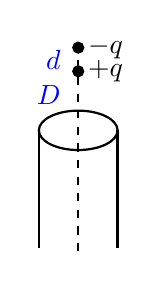
\begin{tikzpicture}
    \draw[thick] (0,0) ellipse (0.5cm and 0.25cm);
    \draw[thick] (0.5,0) -- ++(0,-1.5cm);
    \draw[thick] (-0.5,0) -- ++(0,-1.5cm);
    \draw[thick,dashed] (0,1.1) -- ++(0,-2.7cm);
    \draw[fill=black] (0,0.75) circle (0.07cm) node[right] {$+q$};
    \draw[fill=black] (0,1.05) circle (0.07cm) node[right] {$-q$};
    \draw (-0.1,0.9) node[left,blue] {$d$};
    \draw (-0.1,0.45) node[left,blue] {$D$}; 
  \end{tikzpicture}
}

\taskpic[2.75cm]{ Две тонкие жесткие диэлектрические спицы скреплены и
  образуют угол $2\alpha$. В вершине угла закреплен заряд $-q$. По
  каждой спице может свободно скользить маленькая бусинка заряда
  $+q$. Однородное электрическое поле напряженности $E$ параллельно
  биссектрисе угла. Найдите положения равновесия бусинок. Исследуйте
  устойчивость. Силой тяжести пренебречь. }
{
  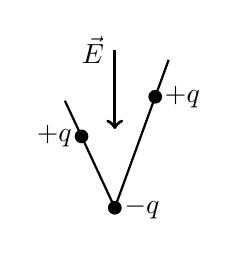
\begin{tikzpicture}
    \draw[thick] (0,0) ++ (115:1.5cm) -- (0,0) -- ++(70:2cm);
    \draw[fill=black] (0,0) circle (0.08cm) node[right] {$-q$};
    \draw[fill=black] (0,0) ++ (115:1cm) circle (0.08cm) node[left]
    {$+q$}; 
    \draw[fill=black] (0,0) ++ (70:1.5cm) circle (0.08cm) node[right]
    {$+q$};
    \draw[very thick,->] (0,2) node[left] {$\vec{E}$} -- (0,1);
  \end{tikzpicture}
}

\taskpic[2.75cm]{ Семь одинаковых зарядов $q$ связаны друг с другом
  одинаковыми упругими нитями так, как показано на рисунке. Расстояние
  между ближайшими зарядами $l$. Определите силу натяжения каждой
  нити. }
{
  \begin{tikzpicture}
    \draw[fill=black] (0,0) circle (0.07cm); 
    \foreach \i in {0,60,120,...,300}
    {
      \draw[thick,fill=black] (0,0) -- (\i:1cm) circle (0.07cm);
      \draw[thick] (0,0) ++ (\i:1cm) -- ($(0,0)+(\i+60:1cm)$);
    }
  \end{tikzpicture}
}

\end{document}


%%% Local Variables: 
%%% mode: latex
%%% TeX-engine:xetex
%%% TeX-PDF-mode: t
%%% End:
